\chapter{Metodologia}

Este capítulo descreve a metodologia adotada na pesquisa, organizada em torno de três decisões centrais: (i) a decomposição da tarefa de conversão de normas para o formato RASE em três níveis sucessivos de normalização (N1, N2 e N3); (ii) o uso de Engenharia de Prompt como técnica de especialização dos modelos; e (iii) a comparação sistemática de seis Modelos de Linguagem de Grande Porte (LLMs) \textit{open-source} servidos localmente via Ollama. O capítulo apresenta também o \textit{dataset} utilizado, o pipeline de execução, os cinco experimentos conduzidos (EN1, EN2, EN1N2, EN3 e EN1N2N3), as métricas de validação e o ambiente computacional empregado.

\section{Visão Geral}

<<<<<<< HEAD
A pesquisa avaliou o uso de LLMs \textit{open-source} para converter normas técnicas da AEC em representações computáveis no formato RASE, utilizando \textbf{exclusivamente Engenharia de Prompt}. A conversão foi modelada como um processo de normalização em três níveis sucessivos: N1 (segmentação atômica das sentenças normativas), N2 (identificação dos operadores RASE) e N3 (estruturação semântica em JSON). Seis modelos LLM foram avaliados sob três experimentos (EN1, EN2 e EN1N2), aplicados a um \textit{dataset} composto por 79 normas brasileiras anotadas, e comparados por meio de treze métricas: nove métricas de similaridade textual (lexicais, semânticas, distância e geração) e quatro métricas de classificação derivadas da matriz de confusão. A Figura~\ref{img:4.1} apresenta uma visão geral do pipeline, do texto bruto à representação RASE final, com indicação dos prompts utilizados em cada nível, do servidor Ollama que hospeda os modelos e da etapa de validação par a par contra o \textit{dataset} de referência.

\begin{figure}[ht]
\centering
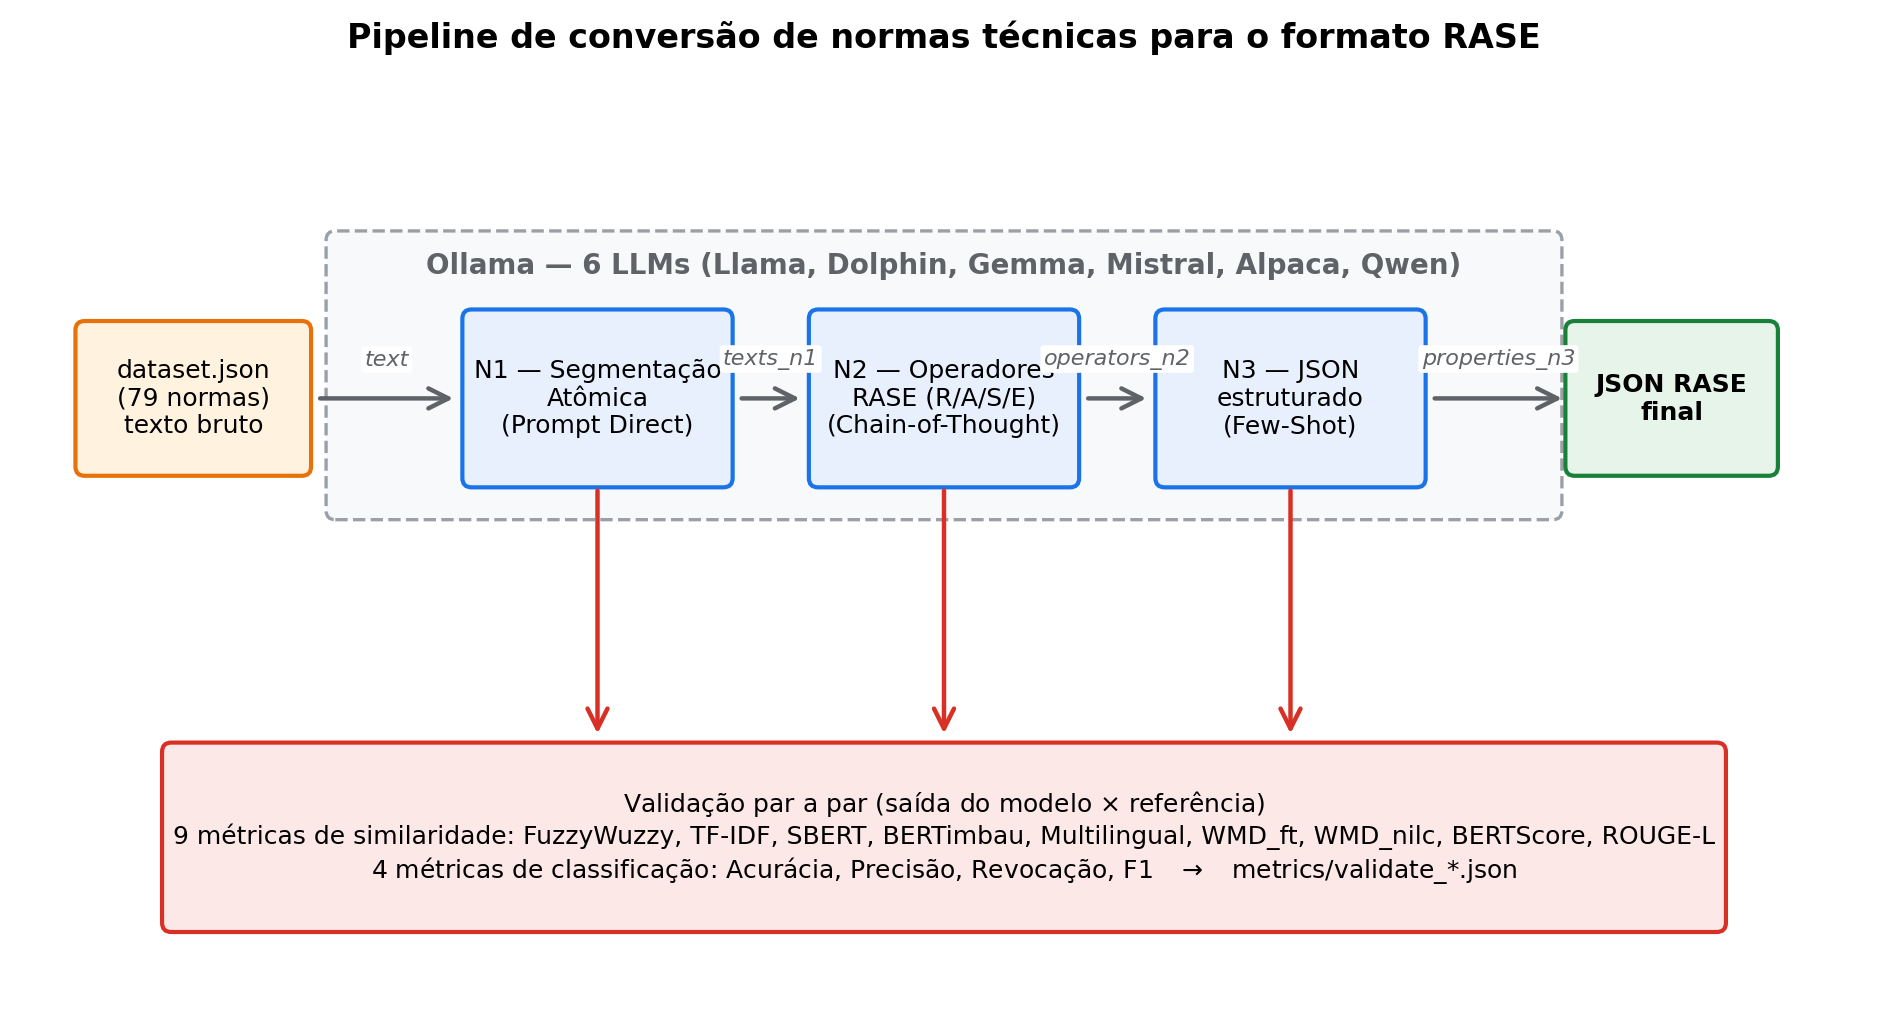
\includegraphics[width=0.98\linewidth]{Imagens/4.1-pipeline.png}
\caption{Pipeline de conversão de normas técnicas para o formato RASE.}
\label{img:4.1}
\end{figure}
=======
A pesquisa avaliou o uso de LLMs \textit{open-source} para converter normas técnicas da AEC em representações computáveis no formato RASE, utilizando \textbf{exclusivamente Engenharia de Prompt}. A conversão foi modelada como um processo de normalização em três níveis sucessivos: N1 (segmentação atômica das sentenças normativas), N2 (identificação dos operadores RASE) e N3 (estruturação semântica em JSON). Seis modelos LLM foram avaliados sob cinco experimentos (EN1, EN2, EN1N2, EN3 e EN1N2N3), aplicados a um \textit{dataset} composto por 79 normas brasileiras anotadas, e comparados por meio de métricas de similaridade textual e de classificação.
>>>>>>> b1bd44c (citation)

\section{Necessidade de Normalização em Três Níveis}

A transformação completa de uma norma técnica em texto bruto para a sua representação RASE final em JSON envolve raciocínios distintos: segmentação sintática, classificação semântica e extração de atributos estruturados. Pedir todas essas decisões em uma única chamada ao LLM tende a degradar a qualidade da saída, induzindo alucinações, omissões e estruturas inválidas. A decomposição em três níveis sucessivos isola cada decisão, mantém cada chamada ao modelo com escopo bem delimitado e permite validar cada etapa independentemente.

\subsection{N1 --- Segmentação Atômica}

Uma sentença normativa frequentemente contém múltiplas regras coordenadas. Por exemplo, o texto ``A inclinação transversal deve ser de até 2\% para pisos internos e de até 3\% para pisos externos'' contém duas regras computáveis distintas. O nível N1 tem como objetivo segmentar a sentença original em sentenças atômicas, em que cada item representa uma única regra. Sem essa segmentação, as etapas subsequentes não conseguem aplicar corretamente os operadores RASE.

O prompt utilizado em N1 é mantido em um arquivo de texto dedicado a este nível e instrui o modelo a quebrar a sentença em sentenças curtas e diretas, uma regra computável por sentença, sem inventar elementos, acompanhado de um exemplo demonstrativo.

\subsection{N2 --- Identificação dos Operadores RASE}

Dada uma regra atômica produzida em N1, o nível N2 tem como objetivo identificar quais trechos correspondem a Requisito (R), Aplicabilidade (A), Seleção (S) e Exceção (E), segundo a metodologia RASE. Essa classificação é o cerne da formalização: sem ela, o texto permanece em linguagem natural.

O prompt N2 é armazenado em um arquivo de texto próprio e define uma ordem fixa para os quatro operadores e um formato exato de saída em quatro linhas, marcando o campo vazio com aspas duplas (\verb|""|). O prompt inclui um exemplo único embutido, que serve de âncora para o modelo.

\subsection{N3 --- Estruturação Semântica em JSON}

Mesmo após classificar um trecho como R, A, S ou E, o conteúdo permanece em linguagem natural. Para que uma regra possa ser verificada automaticamente contra um modelo BIM, é necessário extrair um tripé estruturado composto por \textit{objeto}, \textit{propriedade} e \textit{valor}, complementado por \textit{comparador} e \textit{unidade}. O nível N3 produz esta representação em formato JSON, com os campos \verb|type|, \verb|object|, \verb|property|, \verb|comparation|, \verb|target| e \verb|unit|.

Em função da natureza distinta de cada operador RASE, optou-se por utilizar \textbf{um prompt por operador} em N3, com arquivos de texto separados para Aplicabilidade, Requisito, Seleção e Exceção. A Aplicabilidade descreve \textit{a quem} a regra se aplica; o Requisito descreve \textit{o que} é exigido; a Seleção restringe o escopo; e a Exceção define os casos não cobertos. Cada prompt traz o esquema JSON explícito, regras heurísticas de mapeamento por padrões textuais comuns (por exemplo, ``uso público'' $\rightarrow$ \verb|property "uso", comparation "=", target "público"|) e múltiplos exemplos \textit{few-shot} por operador.

\section{Engenharia de Prompt}

A pesquisa utilizou Engenharia de Prompt como abordagem de especialização. Toda a adaptação dos LLMs à tarefa foi realizada pelo desenho dos prompts, organizados em arquivos de texto dedicados a cada nível e a cada operador. Três técnicas clássicas de Engenharia de Prompt foram aplicadas, cada uma escolhida em função da natureza do nível em que atua.

\subsection{Prompt Direct}

O \textit{Prompt Direct} consiste em uma instrução direta e objetiva, sem encadeamento explícito de raciocínio. Foi aplicado ao nível \textbf{N1}, cuja tarefa --- segmentar uma sentença em sub-regras --- é estruturalmente simples e não exige raciocínio profundo sobre semântica normativa. Suas principais vantagens são o menor consumo de tokens e a menor latência; o risco principal é a queda de robustez diante de sentenças longas ou ambíguas. O prompt N1 consiste em cinco regras imperativas e um exemplo curto, sem instruções de raciocínio passo a passo.

\subsection{Prompt Chain-of-Thought}

O \textit{Prompt Chain-of-Thought} instrui o modelo a explicitar o raciocínio em etapas antes da resposta final. Foi aplicado ao nível \textbf{N2}, em que a classificação de trechos como R, A, S ou E exige a interpretação do papel sintático-semântico do trecho dentro da regra. Esta técnica reduz alucinações e melhora a classificação em sentenças com múltiplos operadores, ao custo de maior consumo de tokens. O prompt N2 apresenta a ordem fixa dos passos (1.~aplicabilidade $\rightarrow$ 2.~seleção $\rightarrow$ 3.~exceção $\rightarrow$ 4.~requisito), guiando o modelo por uma cadeia de decisão explícita.

\subsection{Prompt Few-Shot}

O \textit{Prompt Few-Shot} inclui no próprio prompt exemplos completos de entrada e saída, ancorando o formato esperado. Foi aplicado ao nível \textbf{N3}, em que a saída precisa obedecer a um esquema JSON rígido: sem exemplos, os modelos divergem do formato ou inventam campos. A técnica traz alta aderência ao formato e à terminologia esperada, ao custo de consumir parte da janela de contexto com os exemplos. Cada um dos prompts N3, um por operador RASE, traz de dois a quatro exemplos completos no padrão \textit{operador N2} $\rightarrow$ \textit{JSON}.

\section{Modelos LLM Avaliados}

Seis modelos \textit{open-source} foram servidos localmente por meio do \textbf{Ollama}~\cite{ollama2024} (\texttt{ollama serve}), conforme a Tabela~\ref{tab:modelos_llm}. Todos foram executados sobre o mesmo hardware, com os mesmos prompts e o mesmo \textit{dataset}, garantindo comparabilidade direta entre os resultados. Cinco dos seis modelos correspondem a \textit{checkpoints} adaptados para português brasileiro publicados por terceiros (em especial \texttt{cnmoro/*}, \texttt{splitpierre/*} e \texttt{brunoconterato/*}), todos disponíveis publicamente no registro do Ollama; o Llama foi avaliado em sua versão oficial \texttt{llama3.1:8b}. A coluna \textit{tag} identifica precisamente cada \textit{checkpoint} reprodutível.

\begin{table}[ht]
\centering
\caption{Modelos LLM \textit{open-source} avaliados, com origem e \textit{tag} servida via Ollama (definidos em \texttt{config/models.py}).}
\label{tab:modelos_llm}
\small
\begin{tabular}{llll}
\hline
Modelo & Origem & Tag servida via Ollama & Parâmetros \\
\hline
Llama   & Meta                  & \texttt{llama3.1:8b}                                       & 8B \\
Dolphin & cnmoro (LLaMA-3 PT)   & \texttt{cnmoro/llama-3-8b-dolphin-portuguese-v0.3:4\_k\_m} & 8B (Q4\_K\_M) \\
Gemma   & brunoconterato (PT-BR)& \texttt{brunoconterato/Gemma-3-Gaia-PT-BR-4b-it:f16}       & 4B (FP16) \\
Mistral & cnmoro (PT)           & \texttt{cnmoro/mistral\_7b\_portuguese:q4\_K\_M}            & 7B (Q4\_K\_M) \\
Alpaca  & splitpierre (Bode PT-BR) & \texttt{splitpierre/bode-alpaca-pt-br:13b-Q4\_0}        & 13B (Q4\_0) \\
Qwen    & cnmoro (PT)           & \texttt{cnmoro/Qwen2.5-0.5B-Portuguese-v1:q4\_k\_m}         & 0,5B (Q4\_K\_M) \\
\hline
\end{tabular}
\end{table}

\section{Dataset}

O \textit{dataset} utilizado foi consolidado em um único arquivo JSON, com aproximadamente 270~KB e \textbf{79 normas} anotadas. As normas foram derivadas de regulamentações brasileiras da AEC, com ênfase na NBR~9050 \cite{abnt9050} (acessibilidade a edificações, mobiliário, espaços e equipamentos urbanos), adaptadas a partir do trabalho de Eduardo~\cite{eduardo2020}.

Cada entrada do \textit{dataset} é estruturada da seguinte forma:

\begin{itemize}
    \item \texttt{text}: texto bruto da norma.
    \item \texttt{texts\_n1}: lista de regras atômicas, cada uma com \texttt{text\_n1} e \texttt{operators\_n2}.
    \item \texttt{operators\_n2}: dicionário com as chaves \texttt{requeriments}, \texttt{aplicability}, \texttt{selection} e \texttt{exception}, cada uma com \texttt{text\_n2} e \texttt{properties\_n3}.
    \item \texttt{properties\_n3}: representação em JSON com os campos \texttt{type}, \texttt{object}, \texttt{property}, \texttt{comparation}, \texttt{target} e \texttt{unit}.
\end{itemize}

O mesmo arquivo serve como entrada para os geradores e como \textit{target} de referência para os validadores, simplificando a reprodutibilidade dos experimentos.

\section{Pipeline de Execução e Experimentos}

A orquestração dos experimentos é realizada por um \textit{script} principal, que aciona um menu para a etapa de geração e outro para a etapa de validação. Para cada modelo e para cada experimento, as saídas geradas são persistidas em um arquivo JSON próprio, com o padrão de nomenclatura \texttt{generate\_<nível>\_<modelo>.json} (por exemplo, \texttt{generate\_n1\_alpaca.json} para o nível N1 produzido pelo modelo Alpaca). Os resultados das validações também são armazenados em arquivos JSON dedicados, um por experimento, no padrão \texttt{validate\_<experimento>.json} (por exemplo, \texttt{validate\_n1.json}, \texttt{validate\_n1n2.json} e \texttt{validate\_n1n2n3.json}).

<<<<<<< HEAD
Para isolar as contribuições de cada nível e avaliar a propagação de erros, foram definidos três experimentos, ilustrados na Figura~\ref{img:4.2}. EN1 e EN2 avaliam isoladamente cada etapa --- EN2 utiliza o N1 de referência para eliminar ruído da etapa anterior ---, enquanto EN1N2 simula o pipeline encadeado em que a saída N1 do próprio modelo alimenta sua etapa N2, medindo a propagação de erro.

\begin{figure}[ht]
\centering
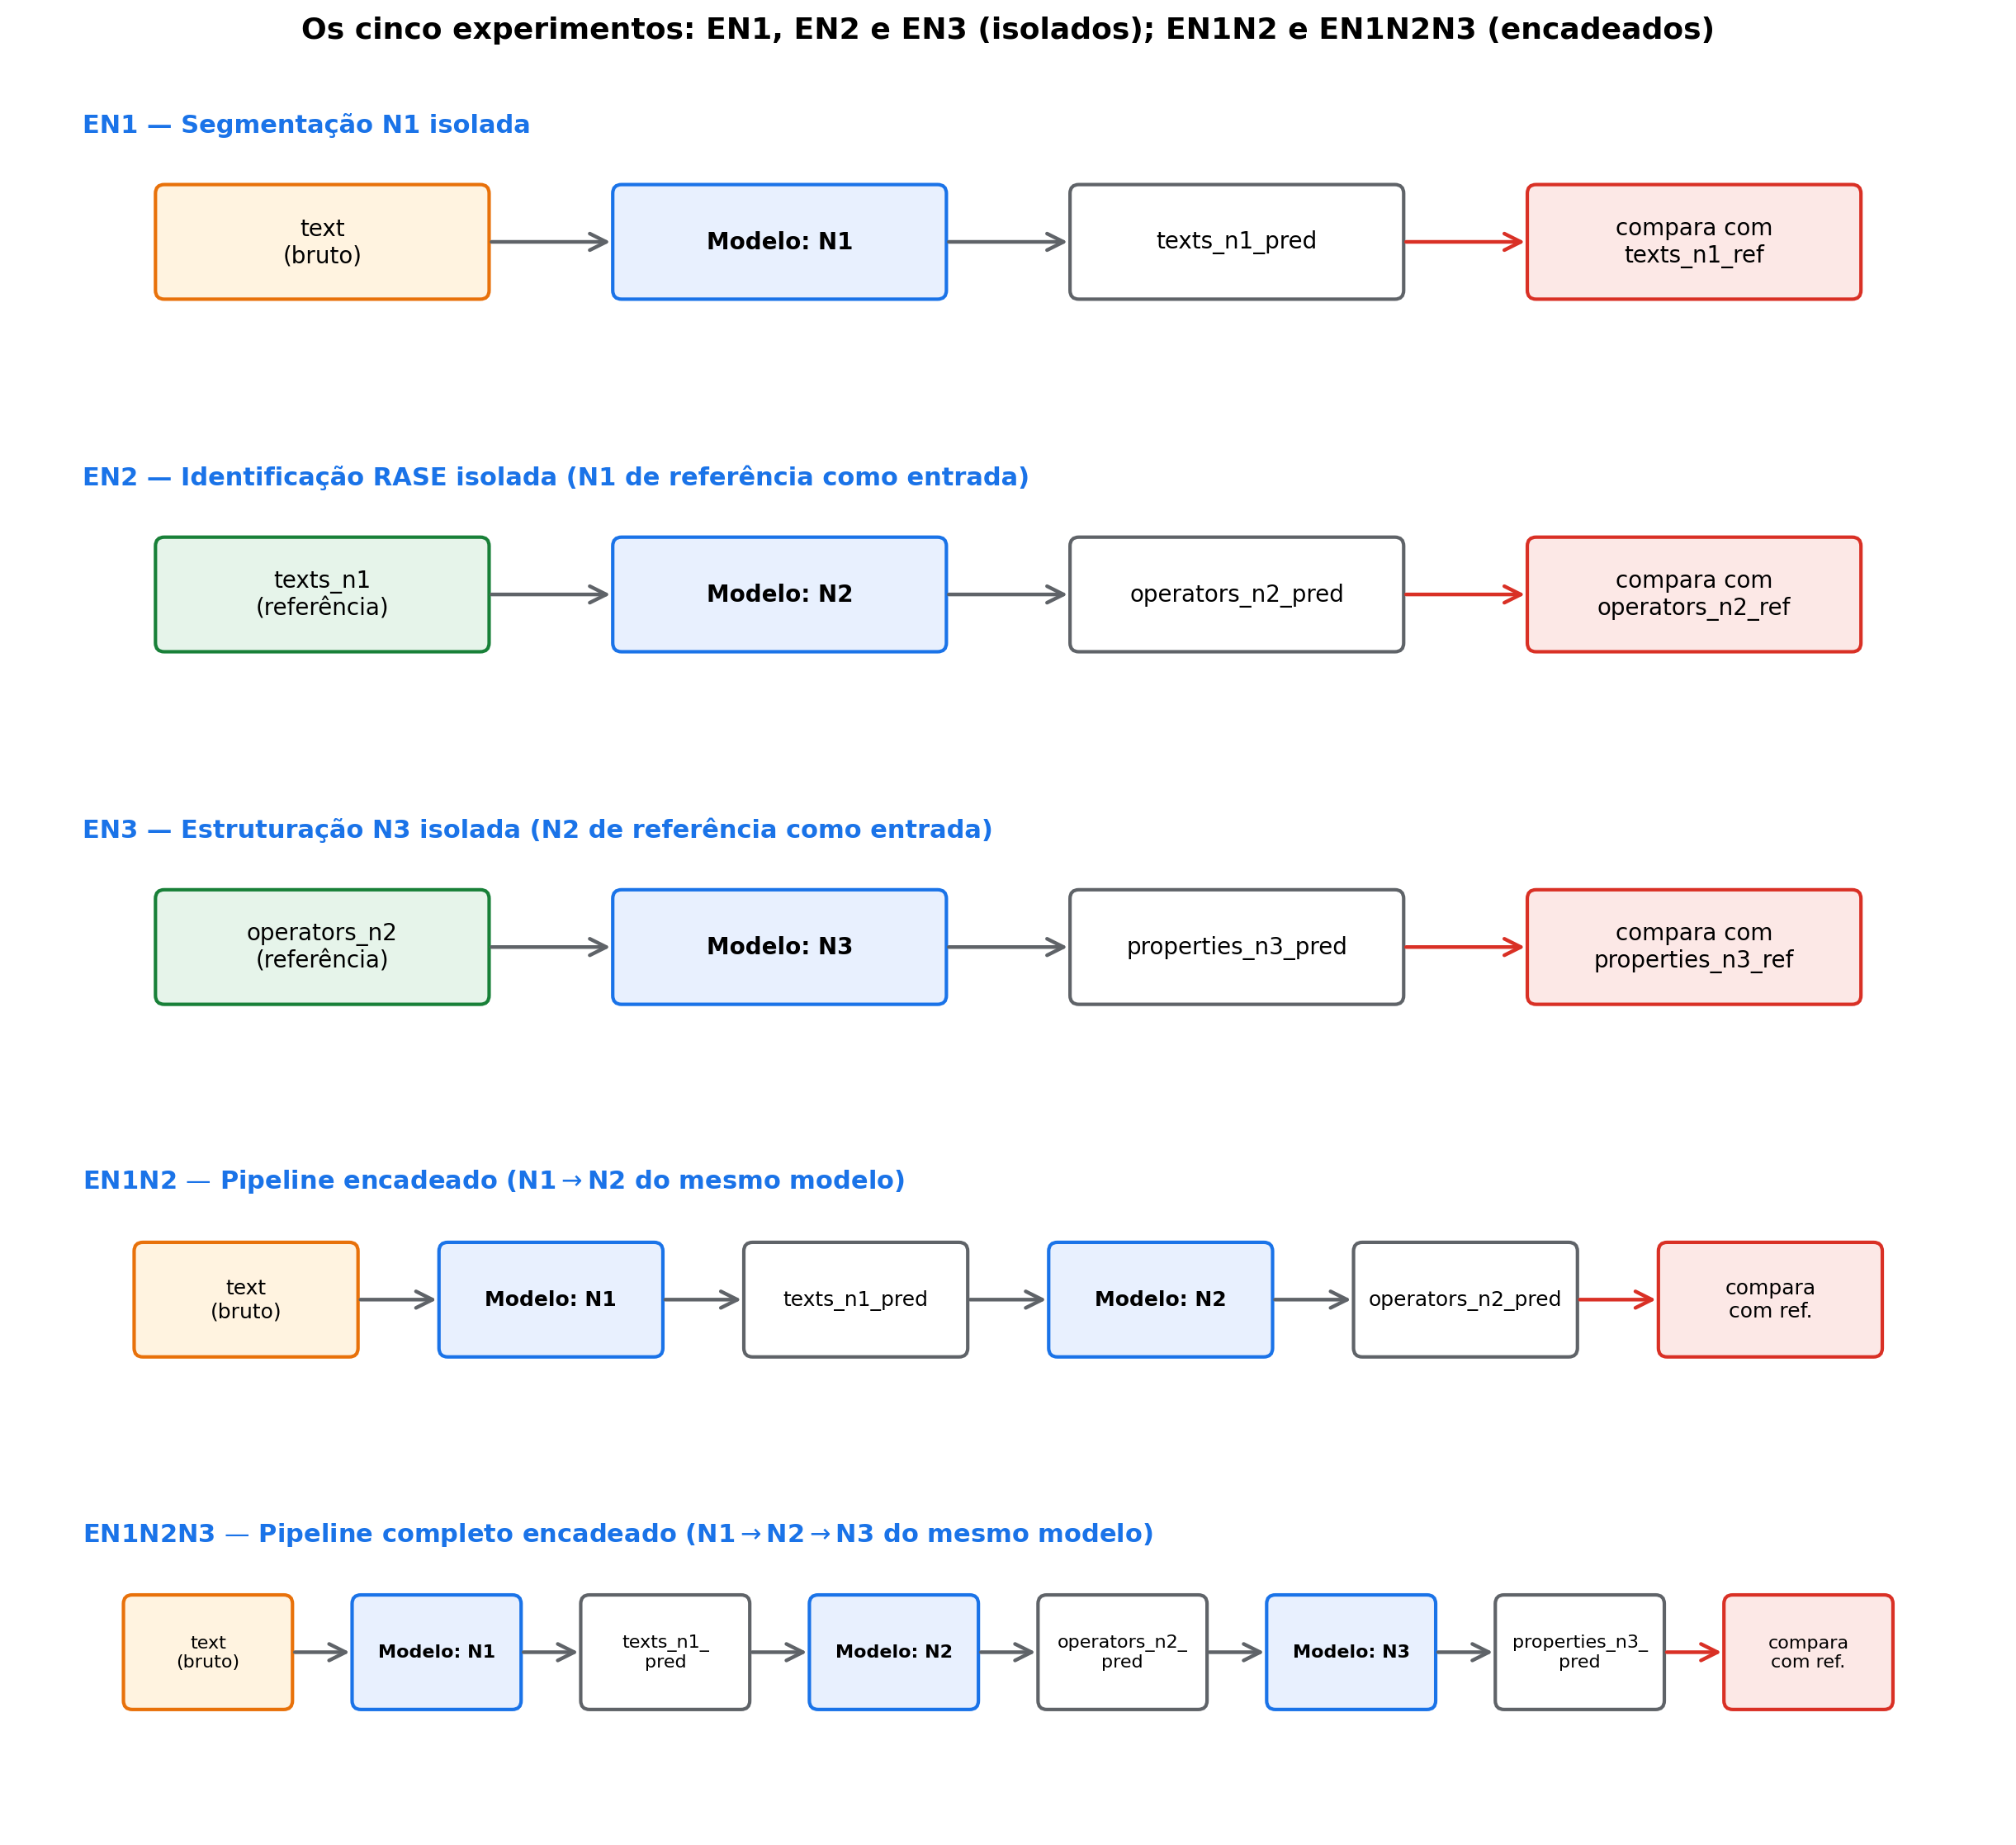
\includegraphics[width=0.98\linewidth]{Imagens/4.2-experimentos.png}
\caption{Estrutura dos três experimentos EN1, EN2 e EN1N2.}
\label{img:4.2}
\end{figure}
=======
Para isolar as contribuições de cada nível e avaliar a propagação de erros, foram definidos cinco experimentos.
>>>>>>> b1bd44c (citation)

\subsection{Experimento EN1}

O experimento EN1 avalia a geração N1 isoladamente. A entrada é o texto bruto da norma, e a saída gerada é comparada ao N1 de referência presente no \textit{dataset}. O experimento mede a qualidade da segmentação a partir do texto bruto, sem influência de etapas posteriores.

\subsection{Experimento EN2}

O experimento EN2 avalia a geração N2 isoladamente, eliminando o ruído proveniente da etapa anterior. A entrada é o N1 de referência (extraído diretamente do \textit{dataset}), e a saída gerada é comparada ao N2 de referência, por operador (R, A, S e E). O experimento mede a qualidade pura da classificação RASE.

\subsection{Experimento EN1N2}

O experimento EN1N2 corresponde ao pipeline encadeado dos dois primeiros níveis: o N1 gerado pelo modelo na primeira etapa alimenta a etapa N2 do mesmo modelo. A saída final é comparada ao N2 de referência. O objetivo é avaliar a \textbf{propagação de erros} entre os dois níveis em um cenário totalmente automatizado.

\subsection{Experimento EN3}

O experimento EN3 avalia a geração N3 isoladamente, eliminando o ruído proveniente das etapas anteriores. A entrada é composta pelo N2 de referência por operador (extraído diretamente do \textit{dataset}), e a saída gerada é comparada à representação JSON estruturada de referência, considerando os campos \texttt{type}, \texttt{object}, \texttt{property}, \texttt{comparation}, \texttt{target} e \texttt{unit}. O experimento mede a qualidade pura da estruturação semântica em JSON, sem influência das etapas de segmentação ou de classificação.

\subsection{Experimento EN1N2N3}

O experimento EN1N2N3 corresponde ao pipeline encadeado completo: o N1 gerado pelo modelo alimenta a etapa N2, que por sua vez alimenta a etapa N3 do mesmo modelo. A saída final --- uma representação em JSON estruturada por operador --- é comparada à referência do \textit{dataset}. O objetivo é avaliar a \textbf{propagação de erros} ao longo dos três níveis em um cenário totalmente automatizado, replicando o uso real do pipeline em produção.

\section{Métricas de Validação}

As saídas dos LLMs foram avaliadas por treze métricas, organizadas em cinco famílias: similaridade lexical, similaridade semântica, distância semântica, métricas voltadas para geração e classificação. As nove primeiras métricas de similaridade são calculadas par a par entre a saída prevista e a referência do \textit{dataset}, em uma escala normalizada $[0,1]$, em que valores mais altos indicam maior similaridade. As quatro métricas de classificação são derivadas da matriz de confusão entre a saída do modelo e a referência.

\subsection{Similaridade Lexical}

\begin{itemize}
    \item \textbf{FuzzyWuzzy}: utiliza \texttt{fuzz.partial\_ratio}, baseado na distância de Levenshtein parcial; tolera fragmentos da string-alvo.
    \item \textbf{TF-IDF}: cosseno entre vetores TF-IDF das duas \textit{strings}, ponderando os termos pela sua importância no corpus \cite{manning2008}.
\end{itemize}

\subsection{Similaridade Semântica}

\begin{itemize}
    \item \textbf{SBERT (PT)}: \textit{embeddings} produzidos pelo modelo \texttt{tgsc/sentence-transformer-ult5-pt-small} \cite{reimers2019}.
    \item \textbf{BERTimbau}: \textit{embeddings} de \texttt{rufimelo/Legal-BERTimbau-sts-large-ma-v3}, especializado em texto jurídico em português brasileiro \cite{souza2020}.
    \item \textbf{Multilingual}: \textit{embeddings} de \texttt{sentence-transformers/paraphrase-multilingual-mpnet-base-v2}, treinado em mais de cinquenta idiomas.
\end{itemize}

\subsection{Distância Semântica (WMD)}

\begin{itemize}
    \item \textbf{WMD\_ft}: \textit{Word Mover's Distance} \cite{kusner2015} com \textit{embeddings} do FastText (\texttt{fasttext-wiki-news-subwords-300}) \cite{bojanowski2017}.
    \item \textbf{WMD\_nilc}: WMD com \textit{embeddings} do projeto NILC (\texttt{cbow\_s300.txt}), treinados sobre corpora em português brasileiro, com valor normalizado para o intervalo $[0,1]$.
\end{itemize}

\subsection{Métricas Voltadas para Geração}

\begin{itemize}
    \item \textbf{BERTScore}: similaridade contextual baseada em \textit{embeddings} do BERT, com alinhamento ótimo entre os \textit{tokens} da saída e da referência \cite{zhang2020bertscore}.
    \item \textbf{ROUGE-L}: razão entre a maior subsequência comum (LCS) e a referência, originalmente proposta para sumarização \cite{lin2004rouge}.
\end{itemize}

\subsection{Métricas de Classificação}

Complementarmente às métricas de similaridade, foram calculadas quatro métricas de classificação. O critério de acerto foi definido em função do nível de normalização:

\begin{itemize}
    \item Em \textbf{N1}, considera-se uma sentença atômica prevista como \textit{verdadeiro positivo} (VP) se sua similaridade semântica em relação a alguma sentença da referência exceder um limiar pré-definido. Como N1 não possui rótulos negativos no \textit{dataset}, calculam-se apenas as estatísticas baseadas em VP, FP e FN.
    \item Em \textbf{N2}, a métrica é calculada por operador (Requisito, Aplicabilidade, Seleção e Exceção) e reporta-se tanto a média macro entre os quatro operadores quanto a média \textit{overall}; o emparelhamento utiliza o mesmo critério baseado em similaridade semântica de N1.
    \item Em \textbf{N3}, a métrica é calculada por campo do JSON (\texttt{object}, \texttt{property}, \texttt{comparation}, \texttt{target} e \texttt{unit}) por correspondência exata, sendo reportada a média macro entre os cinco campos.
\end{itemize}

As métricas são definidas como:

\begin{itemize}
    \item \textbf{Acurácia}: \(\mathrm{ACC} = (\mathrm{VP} + \mathrm{VN})/(\mathrm{VP} + \mathrm{VN} + \mathrm{FP} + \mathrm{FN})\).
    \item \textbf{Precisão}: \(\mathrm{PRE} = \mathrm{VP}/(\mathrm{VP} + \mathrm{FP})\).
    \item \textbf{Revocação}: \(\mathrm{REC} = \mathrm{VP}/(\mathrm{VP} + \mathrm{FN})\).
    \item \textbf{F1-score}: \(\mathrm{F1} = 2 \cdot (\mathrm{PRE} \cdot \mathrm{REC})/(\mathrm{PRE} + \mathrm{REC})\).
\end{itemize}

<<<<<<< HEAD
Todas as métricas são persistidas em \texttt{metrics/validate\_*.json}, e o detalhamento por instância é registrado em \texttt{metrics/details/validate\_<nível>\_<modelo>.jsonl}.
=======
As quatro novas métricas são persistidas no mesmo arquivo de validação de cada experimento, ao lado das métricas de similaridade.
>>>>>>> b1bd44c (citation)

\section{Ambiente Computacional}

Todas as execuções foram conduzidas em uma única estação de trabalho, com a seguinte configuração:

\begin{itemize}
    \item \textbf{CPU}: Intel Core i9-13900K, 13ª geração, 3{,}00~GHz.
    \item \textbf{Memória RAM}: 32~GB.
    \item \textbf{GPU}: NVIDIA RTX 4080.
    \item \textbf{Sistema operacional}: Ubuntu~22.04.
    \item \textbf{Python}: 3.11.9.
    \item \textbf{Servidor LLM}: Ollama (\texttt{ollama serve}).
    \item \textbf{Bibliotecas principais}: \texttt{sentence-transformers}, \texttt{gensim}, \texttt{fuzzywuzzy} e \texttt{scikit-learn} (para TF-IDF).
\end{itemize}

A padronização do ambiente, dos prompts e do \textit{dataset} entre os seis modelos garante que as diferenças observadas nos capítulos seguintes possam ser atribuídas ao comportamento dos LLMs e não a variações de infraestrutura ou de protocolo de avaliação.
